% This is samplepaper.tex, a sample chapter demonstrating the
% LLNCS macro package for Springer Computer Science proceedings;
% Version 2.20 of 2017/10/04
%
\documentclass{llncs}
%
\usepackage{graphicx}

\begin{document}
% Adicionado para por apenas os numeros sem headers
\pagestyle{myheadings}
\title{Development of text-mining solutions to facilitate lipid metabolism interpretation in Genome-Scale Metabolic Models}

\author{Adriano Silva\inst{1}\and
João Ribeiro\inst{1}\and
Emanuel Cunha\inst{1}}

\institute{University of Minho}
%
\maketitle              % typeset the header of the contribution
%
\begin{abstract}
The abstract should briefly summarize the contents of the paper in
15--250 words.

\keywords{First keyword  \and Second keyword \and Another keyword.}
\end{abstract}
%
%
%
\section{Introduction}
\subsection{Context and motivation}
Following the new era of digital development, in the past decades, the whole science is experiencing a great evolution and growth that starts with the investment in education and facilities that ultimately leads to the innovation or the creation of a new "value". 
The exponential growth of the science produced can be measured by the number of articles and citations that are been made through these years\cite{Artigo1}(artigo11).
This is self-evident in the field of omics where the advancement in sequencing techniques and the cost-effectiveness allowed the generation of the so-called Big Data that almost grew by forty times in the last decade \cite{Artigo2}(artigo11). 

Data generated by the multi-omics is extremely useful in the understanding of the different cell 
components as well as in the interactions between them. Systems Biology plays an important 
role in the unveiling of the cellular secrets that are needed to survive and thrive (artigo11/artigo6).
Taking advantage of the multi-omics data gathered, and trying to comprehend the metabolism of a determinated organism,
the construction of genome-scale metabolic models (GSM) took the spotlight. Allowing the seeking for new combinations in the cell network of interactions, this tool as showned useful not only 
to deepen the knowledge of an organism but also to the benefit of the humankind (artigo11/artigo10).

The growing amount and complexity of data generated by multi-omics aligned with the increasing need to have easily accessible, 
well structured and cured data have brought to light some challenges. GSM aproaches integrates all known metabolic information to predict the cellular metabolism and eventually 
trying to optimize the output of a compound with some interest (artigo 10/artigo11). It is therefore imperative to integrate in GSM ----(info atualizada/completa/comprovada. não usar data outra vez)---- that can allow the bests results.
But in fact, the lack of biochemical information in conventional databases is a problem(artigo10). 

In the particular case of Lipids, their representation is often generic
with the lack of structural and biochemical information in the commonly used databases. For this reason, GSM reconstruction does not consider the missing information that is vital to the understanding of the lipids metabolism network.
It is in this niche that a tool capable to integrate specific information of lipids like BOIMMG acts.



\subsection{Objective}
Objetivo proposto para este projeto.
\section{State of art}
\subsection{Omics big data}
O que é o conceito de omica.
\subsection{GSM}
explicar o que é GSM
\subsection{Lipid problem}
Explicar o que é um lipido? e aprofundar o problema.
\subsection{Graph database}
Explicar o que são bases de dados em grafos onde se enquadra a boimmg.

Please note that the first paragraph of a section or subsection is
not indented. The first paragraph that follows a table, figure,
equation etc. does not need an indent, either.

Subsequent paragraphs, however, are indented.

\subsubsection{Sample Heading (Third Level)} Only two levels of
headings should be numbered. Lower level headings remain unnumbered;
they are formatted as run-in headings.

\paragraph{Sample Heading (Fourth Level)}
The contribution should contain no more than four levels of
headings. Table~\ref{tab1} gives a summary of all heading levels.

\begin{table}
\caption{Table captions should be placed above the
tables.}\label{tab1}
\begin{tabular}{|l|l|l|}
\hline
Heading level &  Example & Font size and style\\
\hline
Title (centered) &  {\Large\bfseries Lecture Notes} & 14 point, bold\\
1st-level heading &  {\large\bfseries 1 Introduction} & 12 point, bold\\
2nd-level heading & {\bfseries 2.1 Printing Area} & 10 point, bold\\
3rd-level heading & {\bfseries Run-in Heading in Bold.} Text follows & 10 point, bold\\
4th-level heading & {\itshape Lowest Level Heading.} Text follows & 10 point, italic\\
\hline
\end{tabular}
\end{table}


\noindent Displayed equations are centered and set on a separate
line.
\begin{equation}
x + y = z
\end{equation}
Please try to avoid rasterized images for line-art diagrams and
schemas. Whenever possible, use vector graphics instead (see
Fig.~\ref{fig1}).

\begin{figure}
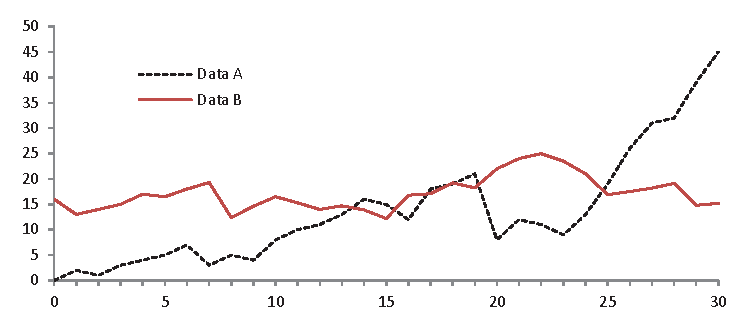
\includegraphics[width=\textwidth]{fig1.eps}
\caption{A figure caption is always placed below the illustration.
Please note that short captions are centered, while long ones are
justified by the macro package automatically.} \label{fig1}
\end{figure}

\begin{theorem}
This is a sample theorem. The run-in heading is set in bold, while
the following text appears in italics. Definitions, lemmas,
propositions, and corollaries are styled the same way.
\end{theorem}
%
% the environments 'definition', 'lemma', 'proposition', 'corollary',
% 'remark', and 'example' are defined in the LLNCS documentclass as well.
%
\begin{proof}
Proofs, examples, and remarks have the initial word in italics,
while the following text appears in normal font.
\end{proof}
For citations of references, we prefer the use of square brackets
and consecutive numbers. Citations using labels or the author/year
convention are also acceptable. The following bibliography provides
a sample reference list with entries for journal


\bibliographystyle{plain}
\bibliography{referencias.bib}
\end{document}
